\documentclass[final]{beamer}
\usepackage[orientation=landscape, size=custom, width=91.44, height=60.96, scale=1.0]{beamerposter}
\usetheme{poster}

\usepackage{amsmath,amssymb}
\usepackage{graphicx}
\usepackage{booktabs}
\usepackage{microtype}
\usepackage{enumitem}
\usepackage{multicol}

% Macros
\newcommand{\Zp}{\mathbb{Z}_{113}}
\newcommand{\POST}{\cPOST}
\newcommand{\PTG}{\cPTG}
\newcommand{\PT}{\cPT}
\newcommand{\eos}{\texttt{eos}}
\newcommand{\WE}{W_E}
\newcommand{\WU}{W_U}
\newcommand{\Wout}{W_{\text{out}}}
\newcommand{\Wlogit}{W_{\text{logit}}}

\begin{document}
\begin{frame}[t]{}

% ============================================================
% TITLE BANNER (dark crimson, matching sample poster)
% ============================================================
\vspace{-1.05cm}
\hspace{-1.05cm}%
\begin{tcolorbox}[
  enhanced,
  width=\paperwidth,
  colback=bannercolor,
  colframe=bannercolor,
  boxrule=0pt,
  arc=0pt,
  left=1.5cm, right=1.5cm, top=0.8cm, bottom=0.8cm,
  boxsep=0pt,
]
  \begin{minipage}[c]{0.82\textwidth}
    {\fontsize{44}{54}\selectfont\bfseries\color{white}
    Do Alignment Pretraining if You Want Your Linear Probes to Work Better ft.\ Modular Addition}\\[20pt]
    {\fontsize{25}{32}\selectfont\color{white}
    Karthik Viswanathan \quad Dmitry Manning-Coe \quad Adam Shai \quad Paul Riechers}
  \end{minipage}%
  \begin{minipage}[c]{0.14\textwidth}
    \centering
    
\includegraphics[height=3.5cm]{logos/mats_white.png}
  \end{minipage}%
\end{tcolorbox}

\vspace{0.4cm}

% ============================================================
% THREE COLUMNS
% ============================================================
\begin{columns}[T]

% ============================================================
% COLUMN 1 — Motivation + Setup + Ensemble
% ============================================================
\begin{column}{0.305\textwidth}

\postersection{Motivation}
\vspace{2pt}
\begin{posterbox}
\posterbody
Alignment via post-training learns a shallow ``wrapper'' over pretrained capabilities (Jain et al., 2024). Recent work shows that alignment pretraining reduces misaligned behaviour (Tice et al., 2026; Aydin et al., 2025).


\vspace{4pt}
\textbf{\textit{If preferences are instead baked into pretraining, does the model develop fundamentally different mechanisms?}} 

\vspace{4pt}
We investigate in a fully interpretable toy model studied in Nanda et al., (2023).
\end{posterbox}

\vspace{12pt}

\postersection{Experimental Setup}
\vspace{2pt}
\begin{posterbox}
\centering
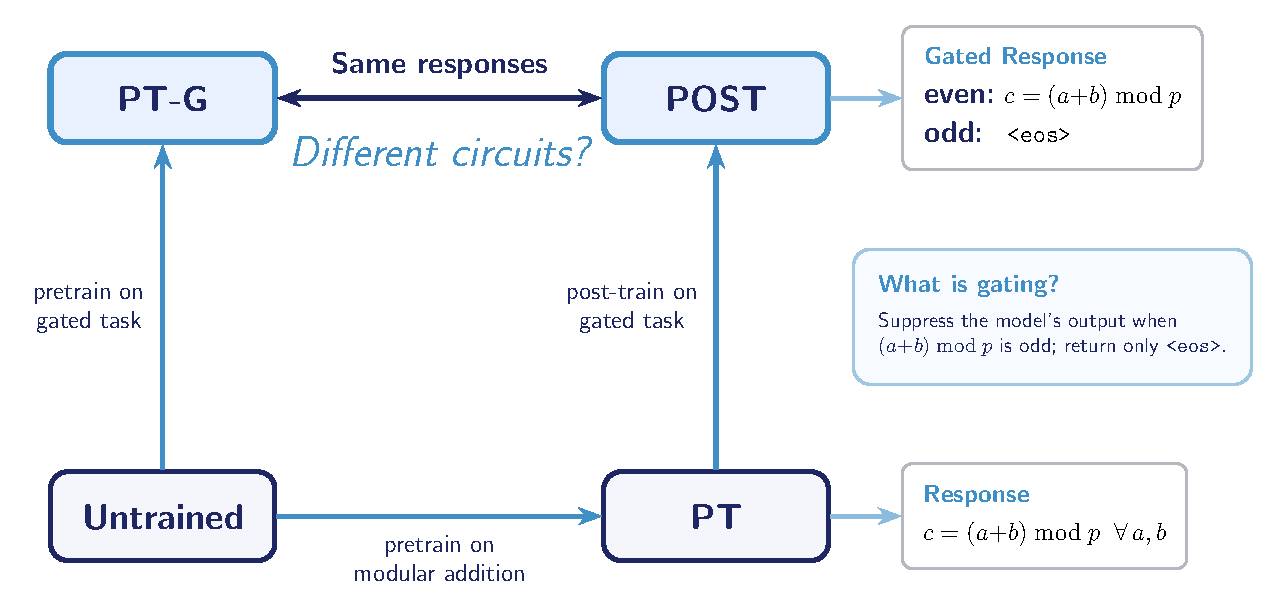
\includegraphics[width=0.95\linewidth]{figs/setup_diagram.pdf}

\vspace{6pt}
\posterbody
\begin{itemize}[leftmargin=*, itemsep=3pt]
  \item \textbf{Task}: Modular addition over $\Zp$ with parity gating
  \item \textbf{Gating}: Even results $\to$ answer; odd $\to$ \eos{} only
  \item \textbf{\POST}: Pretrain on standard task, fine-tune on gated data
  \item \textbf{\PTG}: Train from scratch on gated data
  \item \textbf{Architecture}: 1-layer transformer, 4 heads, $d_{\text{model}}{=}128$
  \item \textbf{Validation}: 126 hyperparameter configurations
\end{itemize}
\end{posterbox}

\vspace{12pt}

\postersection{Ensemble Evaluation}
\vspace{2pt}
\begin{posterbox}
\centering
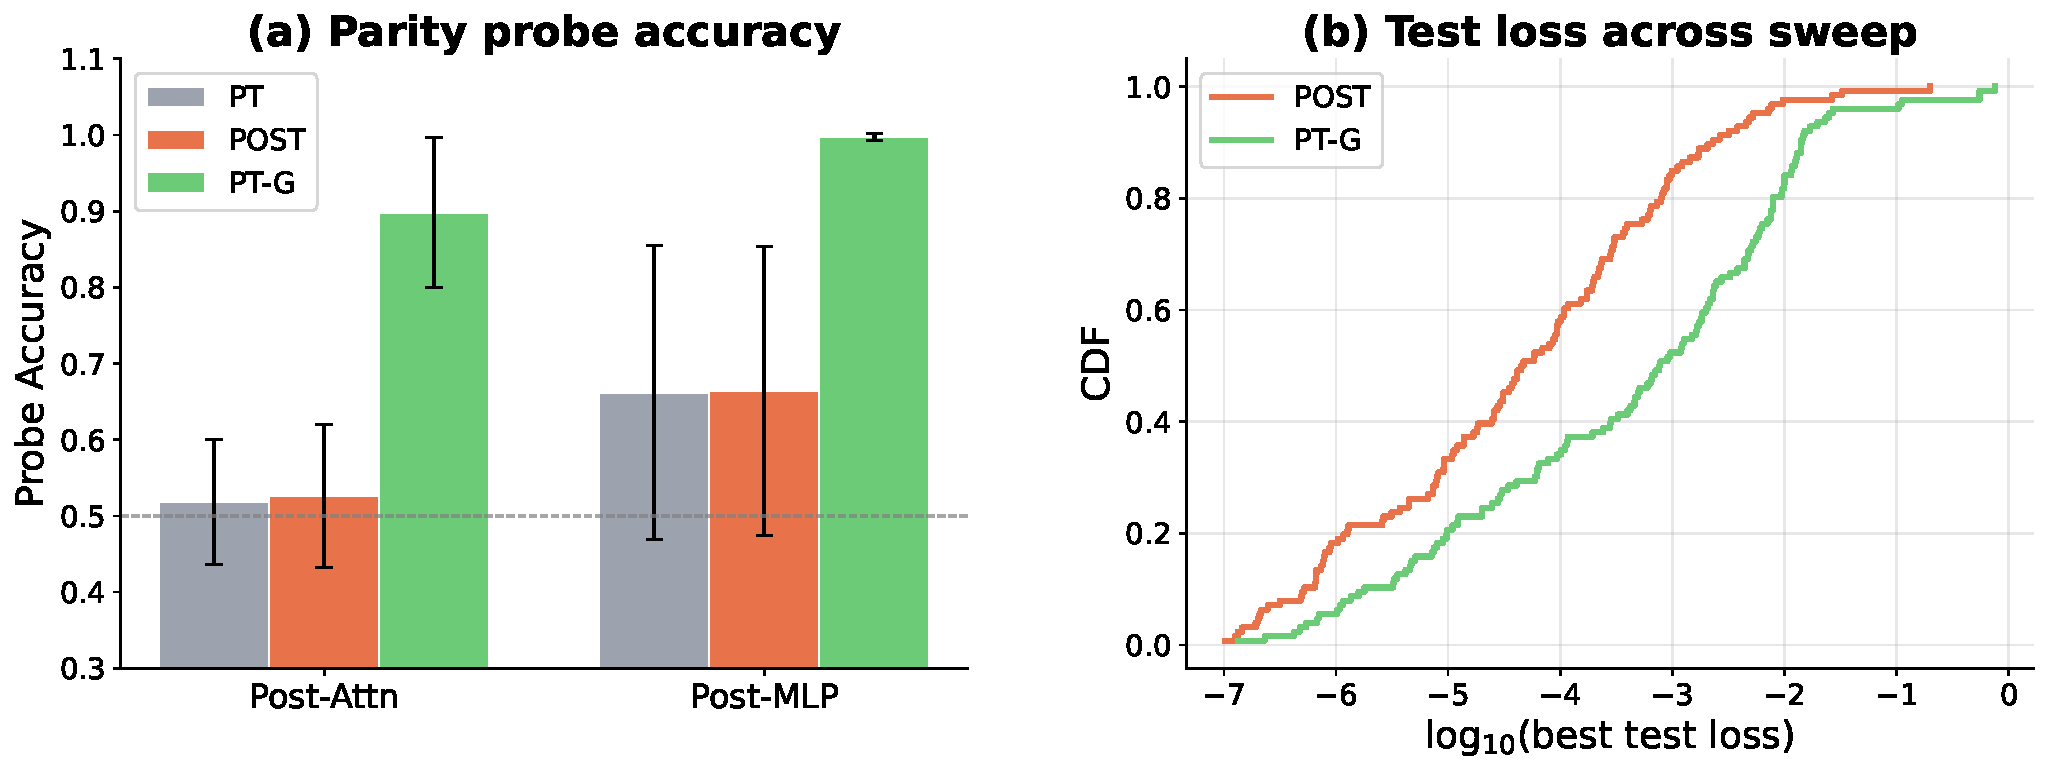
\includegraphics[width=\linewidth]{figs/ensemble_evidence.pdf}

\vspace{4pt}
\posterbody
Across 126 configurations: parity is \textbf{linearly decodable} in \PTG's residual stream but \textbf{not} in \POST{} or \PT.
Meanwhile, \POST{} consistently achieves \textbf{lower test loss} than \PTG{} --- a capability tax for deeper alignment.
\end{posterbox}

\end{column}

% gutter
\begin{column}{0.0175\textwidth}\end{column}

% ============================================================
% COLUMN 2 — Canonical Model Deep Dive
% ============================================================
\begin{column}{0.305\textwidth}

\postersection{Residual Stream Geometry}
\vspace{2pt}
\begin{posterbox}
\centering
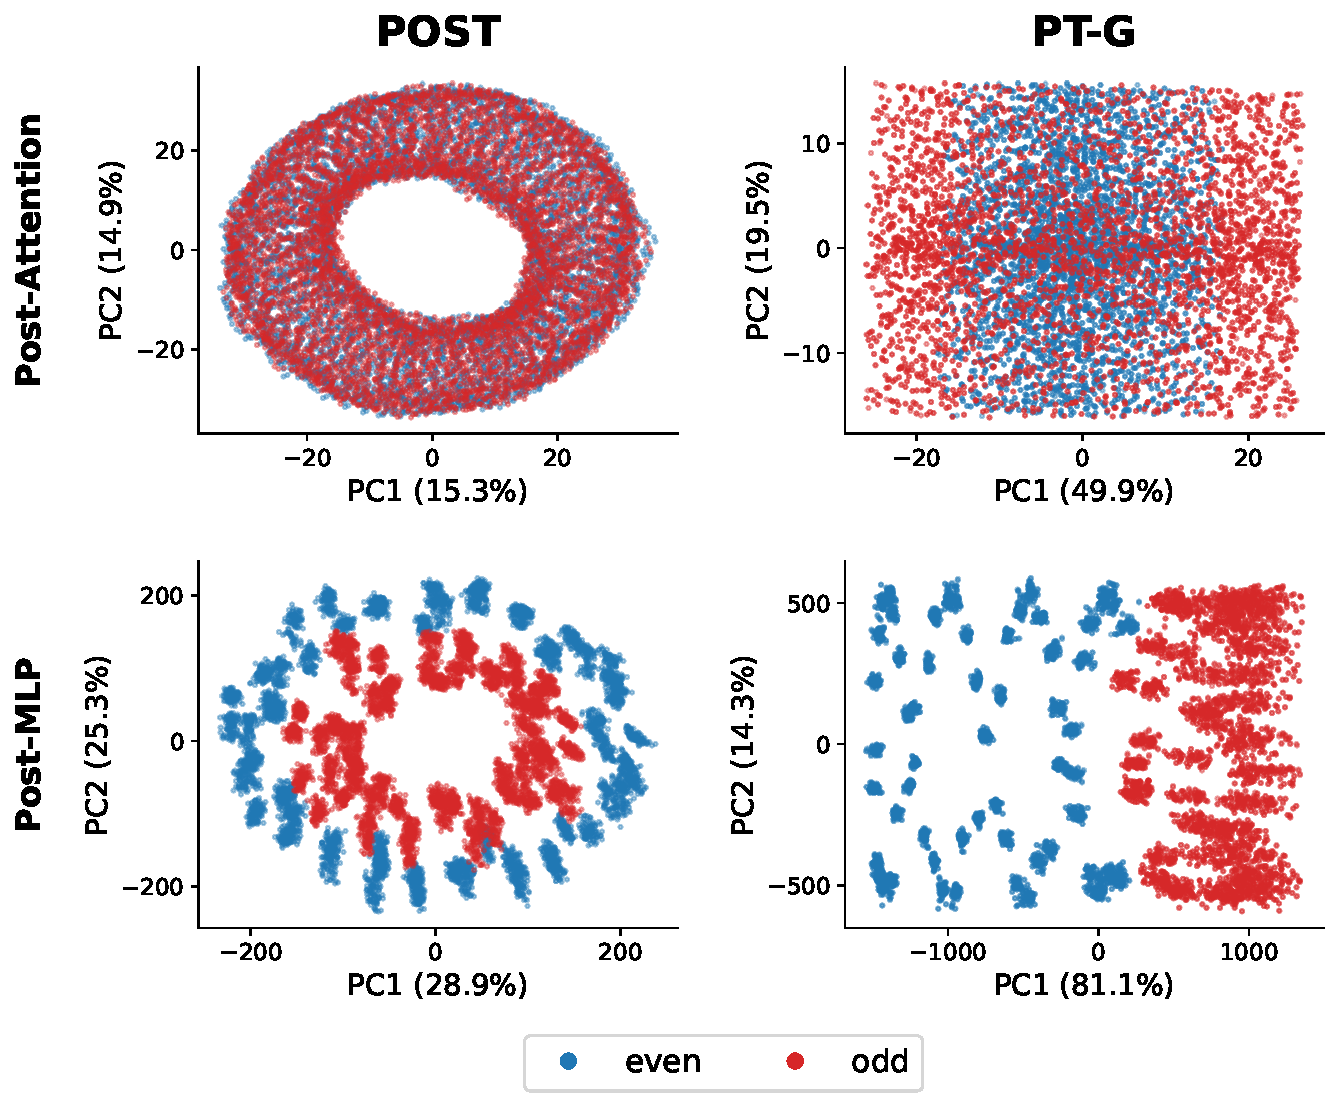
\includegraphics[width=0.95\linewidth]{figs/pca_comparison.pdf}

\vspace{2pt}
{\fontsize{18}{22}\selectfont
PCA at the \texttt{=} token.
\POST{} preserves the \textbf{Fourier ring} (even/odd interleaved);
\PTG{} \textbf{separates even and odd} along top PCs.}
\end{posterbox}

\vspace{4pt}
\postersection{Fourier Analysis}
\vspace{1pt}
\begin{posterbox}
\centering
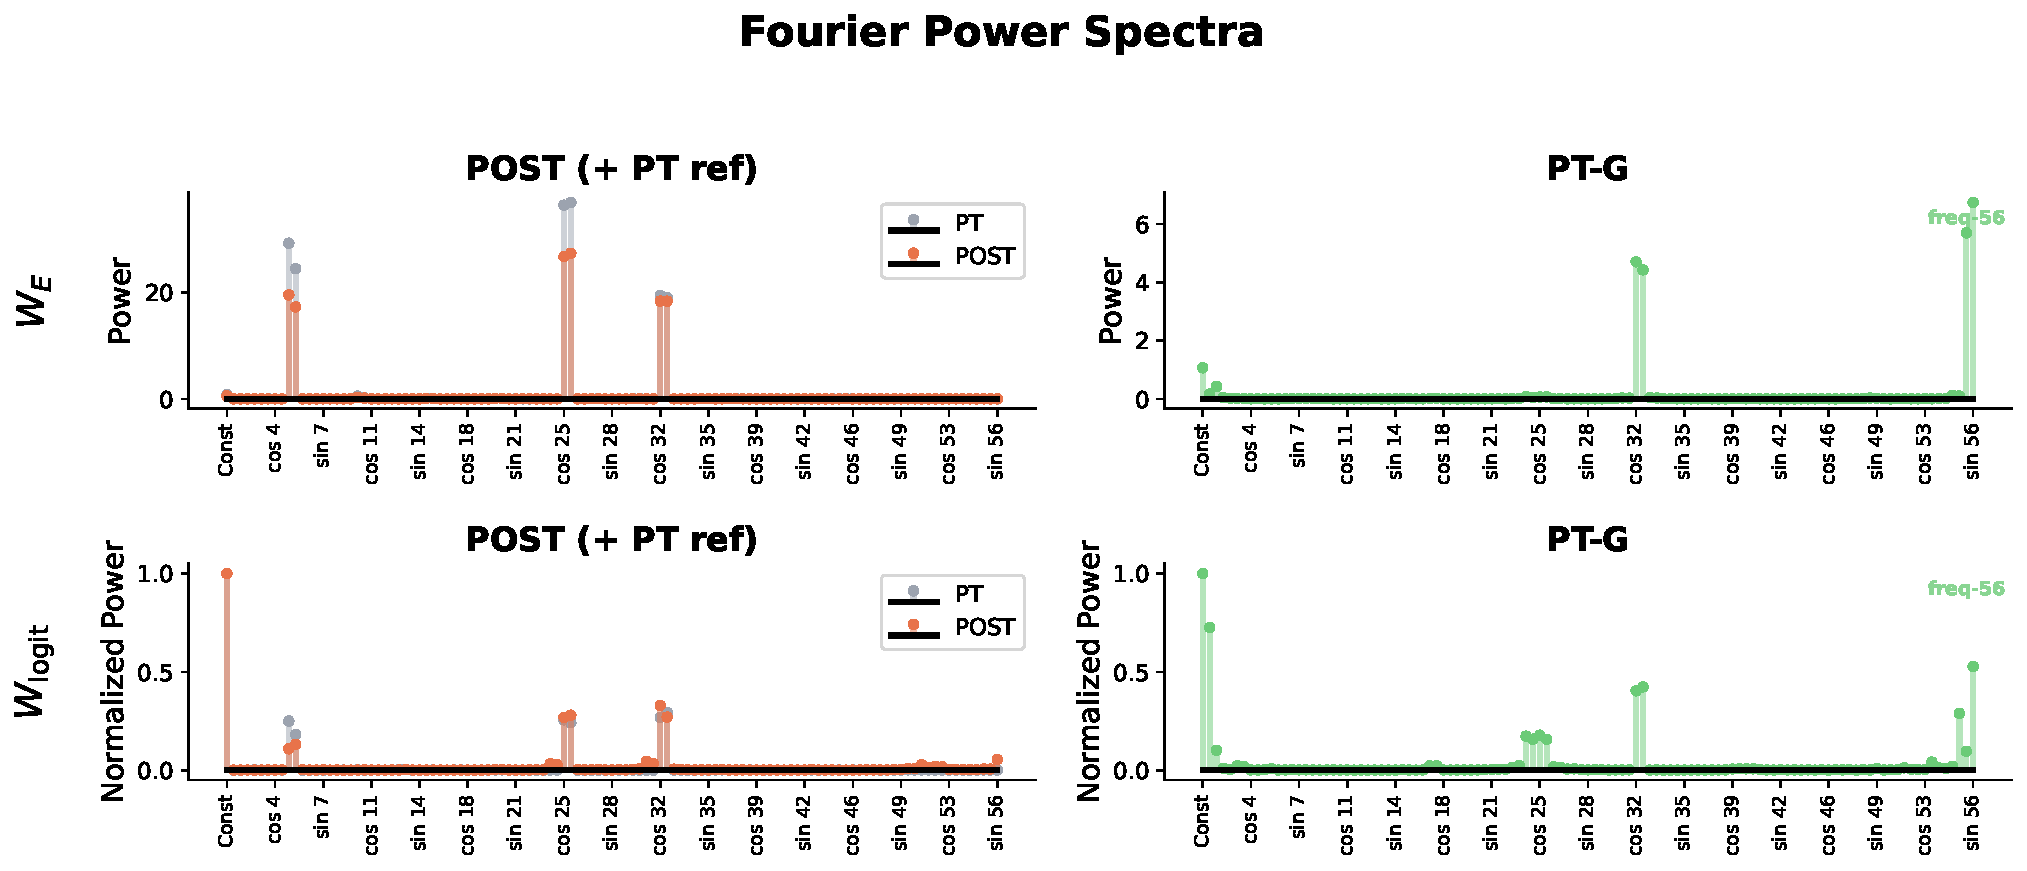
\includegraphics[width=0.95\linewidth]{figs/fourier_combined.pdf}
\vspace{1pt}

{\fontsize{17}{21}\selectfont
\POST{} preserves \PT's peak frequencies in $\WE$ and $\Wlogit$.
\PTG{} develops \textbf{freq-56} (${\approx}(-1)^n$, parity proxy).}
\end{posterbox}

\end{column}

% gutter
\begin{column}{0.0175\textwidth}\end{column}

% ============================================================
% COLUMN 3 — Probes + Implications
% ============================================================
\begin{column}{0.305\textwidth}

\postersection{Parity Probes (Canonical Model)}
\vspace{2pt}
\begin{posterbox}
\centering
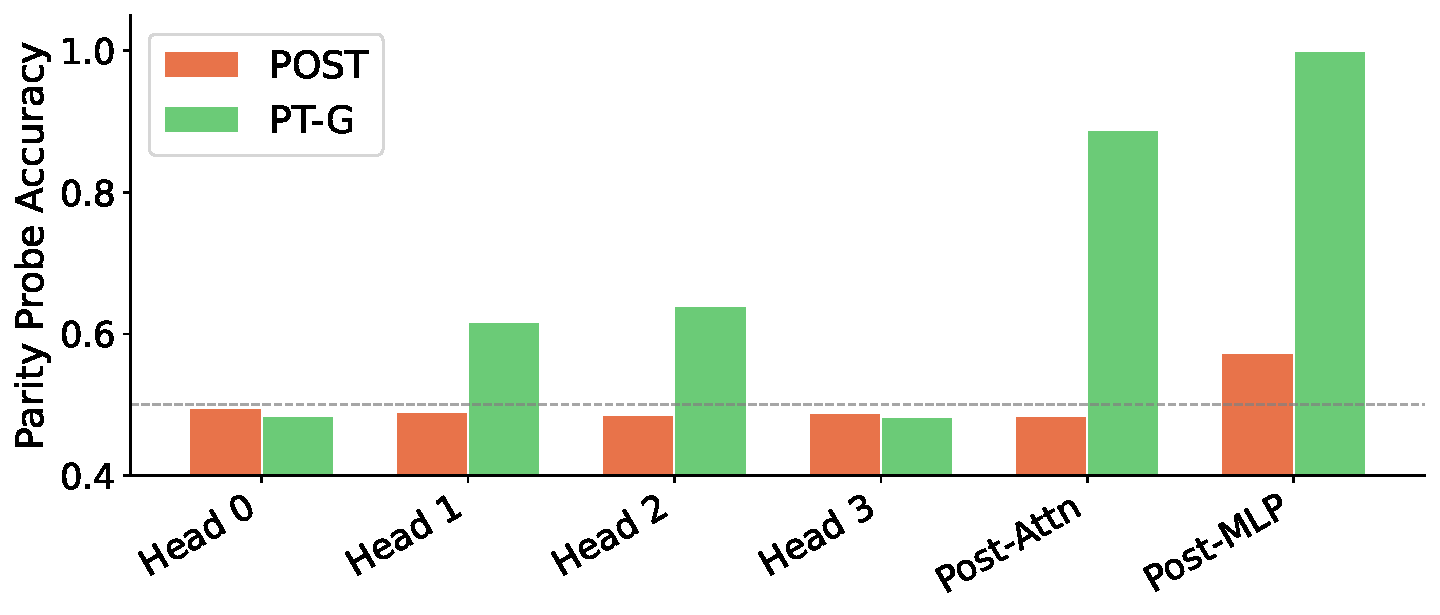
\includegraphics[width=\linewidth]{figs/probe_bars.pdf}

\vspace{4pt}
\posterbody
Linear parity probe accuracy at six network locations.
\PTG{} encodes parity \textbf{progressively}: $62\%$ in heads $\to$ $89\%$ post-attn $\to$ $100\%$ post-MLP.
\POST{} remains at \textbf{chance} (${\sim}50\%$).
\end{posterbox}

\vspace{10pt}

\postersection{Beyond Linear Probes}
\vspace{2pt}
\begin{posterbox}
\centering
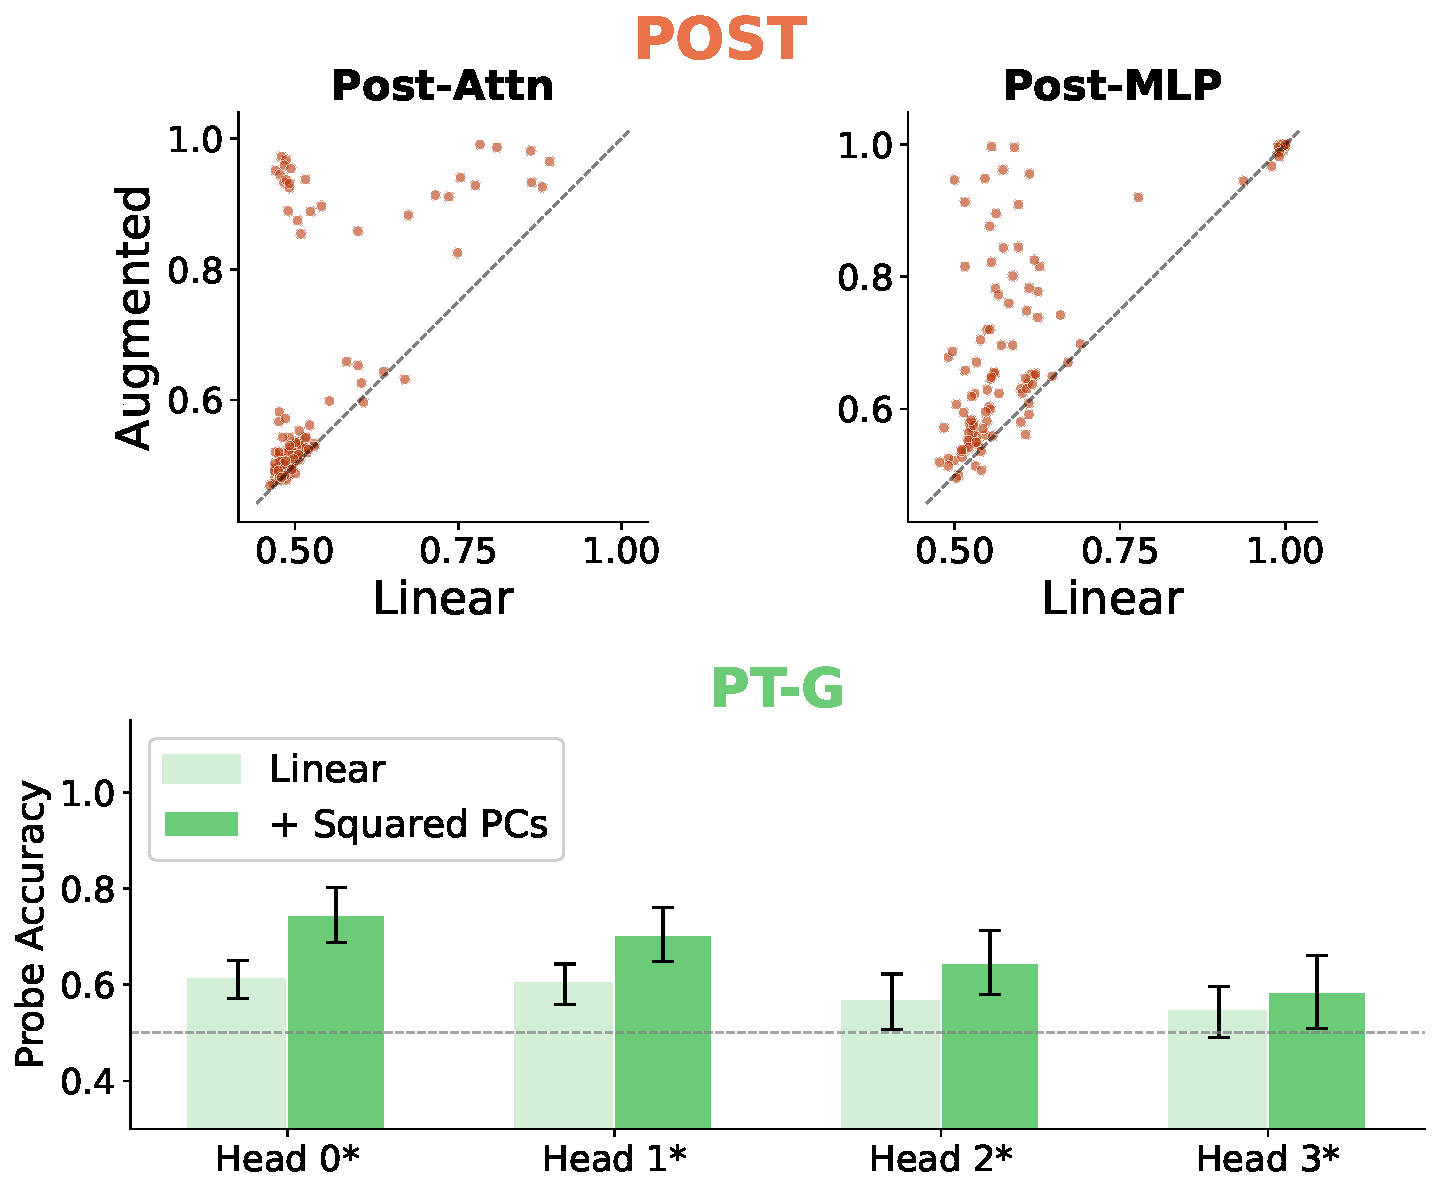
\includegraphics[width=\linewidth]{figs/augmented_probes.pdf}

\vspace{4pt}
\posterbody
Adding squared PC features reveals \POST{} encodes parity \textbf{nonlinearly}
(post-MLP: $0.57 \to 0.96$), consistent with the ring geometry.
\PTG{} is already at ceiling.
\end{posterbox}

\vspace{12pt}

\postersection{Key Takeaways}
\vspace{2pt}
\begin{takeawaybox}
\posterbody
\begin{itemize}[leftmargin=*, itemsep=6pt]
  \item \textbf{\POST{} = shallow output-layer patch} preserving pretrained Fourier circuits. Alignment is achieved by modifying only the unembedding, not the internal computation.
  \item \textbf{\PTG{} = deep structural integration} of preferences throughout the network. Parity is encoded from embeddings through the MLP.
  \item \textbf{White-box probes work better on alignment-pretrained models.} Linear probes can detect preference encoding in \PTG{} but not \POST{} --- relevant for monitoring deployed systems.
\end{itemize}
\end{takeawaybox}

\vspace{12pt}

{\posterref
\textbf{References}\\[3pt]
\begin{enumerate}[leftmargin=*, itemsep=1pt, label={[\arabic*]}]
  \item Jain et al.\ (2024). ``Mechanistically analyzing the effects of fine-tuning on procedurally defined tasks.'' \textit{ICLR}.
  \item Aydin et al.\ (2025). ``From model training to model raising.'' \textit{Communications of the ACM}.
  \item Tice et al.\ (2026). ``Alignment pretraining: AI discourse causes self-fulfilling (mis)alignment.'' \textit{arXiv:2601.10160}.
  \item Nanda et al.\ (2023). ``Progress measures for grokking via mechanistic interpretability.'' \textit{ICLR}.
\end{enumerate}
}

\end{column}

\end{columns}

\end{frame}
\end{document}
